\documentclass[11pt]{article}

\usepackage{graphicx}

\title{\textbf{JDBC Project Final Submission Report \\ Best Bus-path Finder}}

\usepackage[left=1.2in,top=1.0in,right=1.2in,bottom=1.0in]{geometry} % Document margins
\author{Rohit Kumar \\ Roll No. 120050028
		\and
		Rakesh Ranjan Nayak \\
		Roll No. 120050047\\
		\and
		Suman Sourabh \\
		Roll No. 120050031}
\date{\today}
\begin{document}

\maketitle

\section{Introduction}
\paragraph{}

This report talks about a database based web application to facilitate a bus transport system. The applications provides support for searching different types of buses at a particular duration of day and gives the time taken by the buses in the journey. It also provides facilities for registering a new bus in the transport network through an interactive interface. Also, special support for registered users are provided. This includes various discounts which are provided through them through a mathematical discount model.

The entire project is based on an Entity-Relationship model and is strictly followed during the application execution. The database operations are supported by a postgreSQL database engine at the back-end and several other web functionalities like jQuery, AJAX, jsp etc. are used to facilitate interaction with user. Several optimizations in database context has been done by normalization, indexing and analysing the execution plan.


\section{Structure and design of the application}
\paragraph{}
The several servlets/classes used in the applications are described as follows:

\subsection{Main Servlet class}
\paragraph{}
This class establishes connection with the database and handles requests ranging from login to logout, sign up, bus registry, bus search and  payment transaction. This class de-multiplexes the various requests to different classes.

\subsection{Login Check class}
\paragraph{}
This class handles login requests. On every session, a new HTTP session is created and it stores the actions performed by the user during the period it is logged in. This also shares some data structures used by different classes for performing operations related to a particular session. For e.g. a Hash Map is used for storing the bus stops enlisted in a new bus registry to avoid formation of loops.

\subsection{Logout Handler class}
\paragraph{}
Destroys (invalidates) the HTTP session and the user is logged out.

\subsection{Sign Up class}
\paragraph{}
Signs up a new user. Asks for a user-name, password and password confirmation. Checks if the username is already in the database or not and whether the password and it's confirmation are same.

\subsection{Transactions Class}
\paragraph{}

This class is used for generating the list of eligible buses for a source, destination pair, the requested time of starting journey etc. This servlet is executed upon a POST request send by the client using AJAX. The execution plan of this class is described as:
\begin{itemize}
\item Firstly, the list of buses that pass through both the source and destination are obtained 
\item For every such bus, their entire routes and starting time of the bus at it's initial bus stop are obtained. Now, considering the \textbf{traffic} at a particular time of the day, it's expected time to arrive at the source is calculated. If this time falls within the time window provided by the user, then this bus is put in the list of eligible buses. 

\item For calculating the expected time the traffic array stored in the database is used for a particular path, i.e. for very pair of adjacent nodes, the expected time of travel is the traffic value at that particular time of the day 

\end{itemize}
\subsection{Bus Registry Class}
\paragraph{}

This class provides the functionality to register a new bus. This is also supported by an AJAX client interface. This facility can be accessed only by registered users and not by everyone. The admin performing the registry first enters the source of the bus. Then the registry interface provides the adjacency list of the source, i.e. the list of bus stops which are directly connected by the source. The admin can now select the next hop from only these users. 

While the list of the bus stops are being entered by the user, it is ensured that if a bus has already been entered by the user then it is not eligible for being in the bus route by storing every added bus stop in the route in a \textbf{hash map}.

\subsection{guest.jsp}
\paragraph{}

This jsp file handles all client side codes with respect to login, signup, session handling, logout, bus searches and making transactions and  the  connection to the web servlets. All utilities are handled in the same page by using modal popups. 

We are also implementing get and post requests to the servlets are effectively handled using ajax in main.js which interacts with the server code without having to reload the page. 


\subsection{busRegistry.jsp}
\paragraph{}

This file are for bus owners who want to register their buses with the system. This has the facility to automatically suggest the admin the next possible stops which can be inserted from the bus stops adjacency list of the corresponding bus stops he just entered. For stopping the user from entering the inputs he has previously entered we are disabling inputs which have already been taken.  

Here we have implemented way of inserting  new inputs for bus stops in routes. If the route is not registered currently we are updating our route table from the route information given by the user.


\subsection{Other External API's}
\paragraph{}
For an elegant user experience, we have used the Bootstrap \cite{bstrap} library. We have also used jQuery\cite{jquery} for simplifying the scripting of web pages.

\section{AJAX}

\subsection{Auto Completion} 

\paragraph{}	
The Auto completion feature for the  bus stop searches are implemented by sending ajax requests to the servlet class AjaxHandler which returns the possible bus stop names which starts with the input provided by the user. Upon clicking any of the bus stop from the bus stop list the input value is being filled with that bus stop name.

\subsection{Bus search} 

\paragraph{}	

Bus searches are made using ajax to transactions class which gives all buses which are going through these the bus stops within a framework of time given by the user.  The response from the server is sent via json to the ajax handler in main.js which then inserts into the search page in a nice way. 

\begin{figure}[ht!]
\center
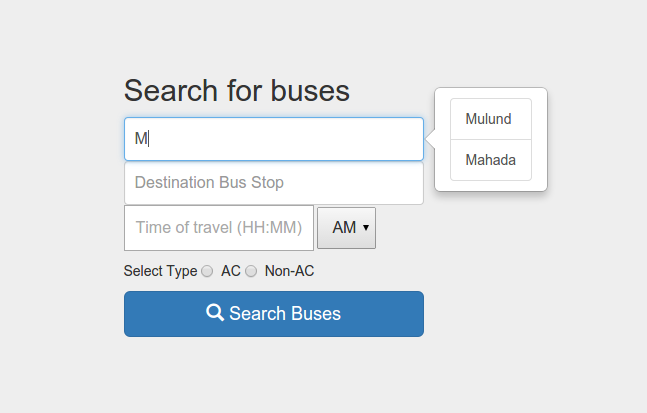
\includegraphics[scale = 0.70]{shots/bussearch.png}
\caption{AJAX Requests for auto completion}
\label{overflow}
\end{figure}

\subsection{Next Bus stops in route in bus registry} 

\paragraph{}	

The adjacency list of the bus stop entered by the user is shown to the user using select lists which are fetched from the server using AJAX which forms a convenient way to insert route without the user having to care for impossible paths. 

\begin{figure}[ht!]
\center
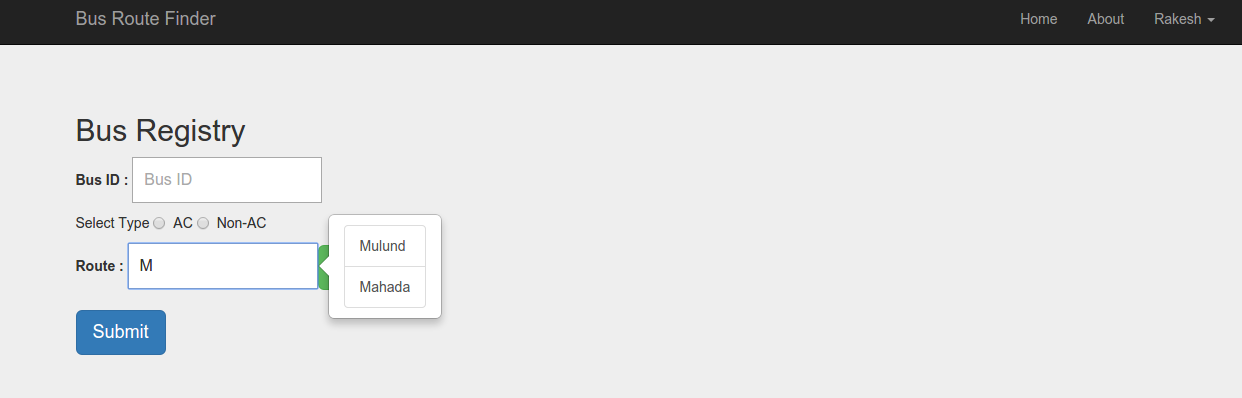
\includegraphics[scale = 0.36]{shots/ajaxreq.png}
\caption{AJAX Requests for auto completion}
\label{overflow}
\end{figure}


\section{Application Architecture}

\subsection{Database Normalization}
\paragraph{}

We have broken down the database into many tables which conserve BCNF database normalization i.e. those attributes which implies other attributes in a table using functional dependency are either candidate keys for those relations or the dependency is trivial. 

For example in paths table, 
\begin{enumerate}
\item (src\_id,dst\_id) $\rightarrow$ path-id and 
\item (src\_id,dst\_id) $\rightarrow$ (ticket\_ac, ticket\_non\_ac,time\_to\_travel, traffic\_rate) 
\end{enumerate}
(src\_id,dst\_id) is also a candidate key for the table paths. There are no such other functional dependencies which are neither trivial nor violates  candidate key constraint. So, It does not violate BCNF normalization.  

\subsection{Indexing}
\paragraph{}
For searching buses, as we have to access records in the bus\_stop table using bus\_stop\_name more often, we have created index on bus\_stop\_name on the table bus\_stops. Similarly as searching for routes while inserting buses into a route is frequent, We have created index on routes(list\_buses).


\section{Interface Design}
\paragraph{}
The following interfaces will be enabled to interact with the user:

\begin{enumerate}
\item \textit{The introductory page will consist of these options:}
\begin{itemize}
\item  \textbf{Proceed as guest and book a journey}

This page which will take various inputs required for providing them the list of travel options.

\begin{figure}[ht!]
\center
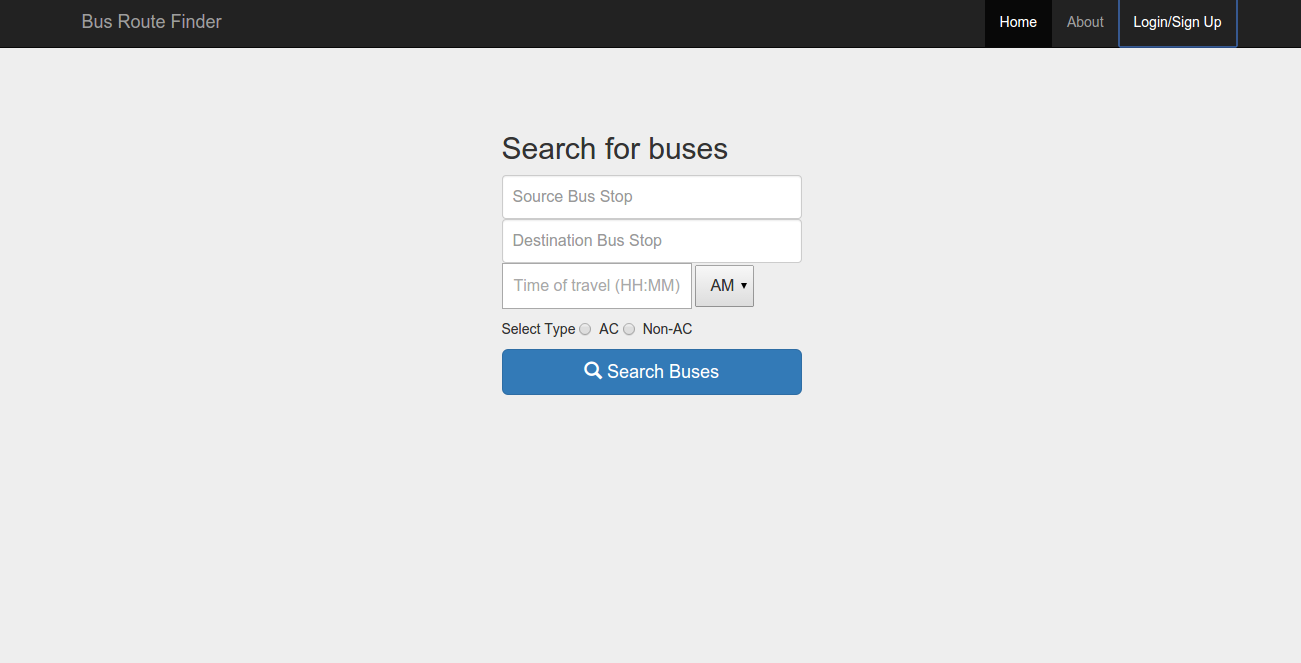
\includegraphics[scale = 0.36]{shots/guest.png}
\caption{The transaction page for a guest user}
\label{overflow}
\end{figure}


\item \textbf{Login Page}

The login page will have input fields of user-name and password as usual. 

\begin{figure}[ht!]
\center
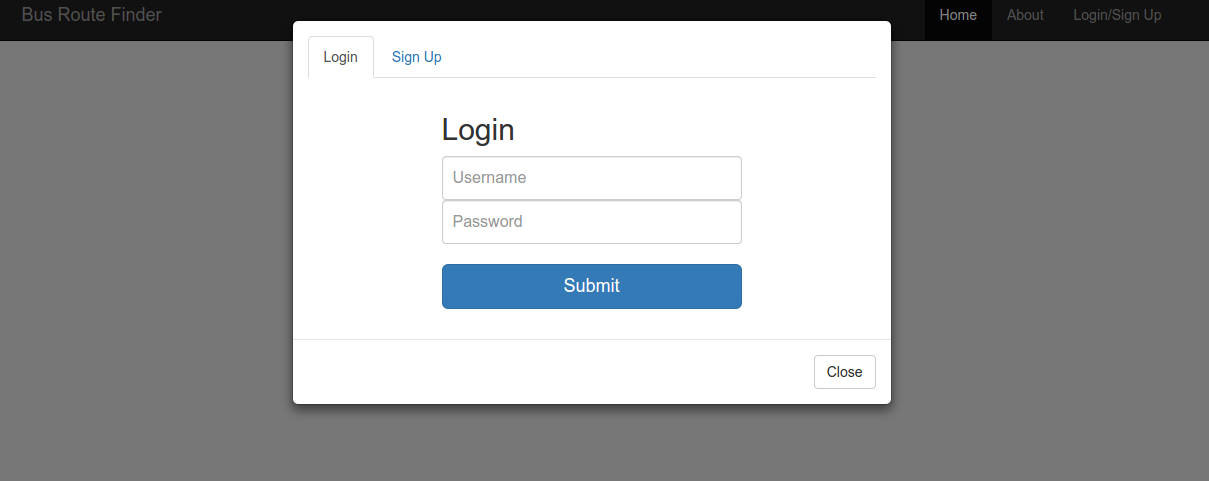
\includegraphics[scale = 0.4]{shots/login.png}
\caption{The transaction page for a guest user}
\label{overflow}
\end{figure}


\item \textbf{Login as a user and book a journey}

Upon successful login, it will create a new user session and redirect the user to a modification of the above page i.e. apart from the above options, it will have the favorite routes (i.e. most traveled routes), according to his/her previous transactions. This will make the transaction process easy for the user.

\begin{figure}[ht!]
\center
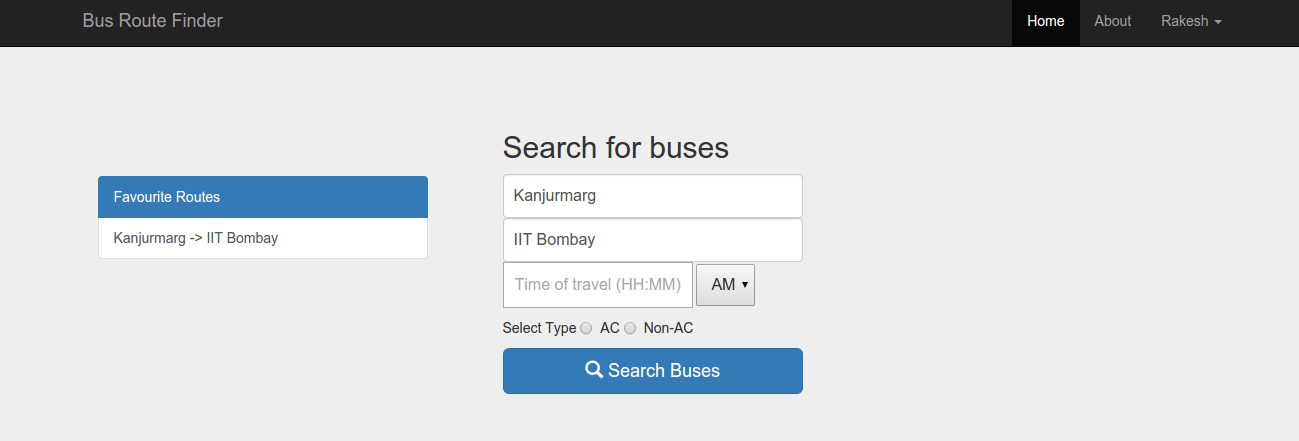
\includegraphics[scale = 0.36]{shots/favroutes.png}
\caption{The transaction page of a registered user with his/her favorite routes}
\label{overflow}
\end{figure}



\item \textbf{Register as a new user} 

This will enable the registry of a new user. It will ask for the various input fields required i.e. a unique user-name, password and a confirmation of it.

\begin{figure}[ht!]
\center
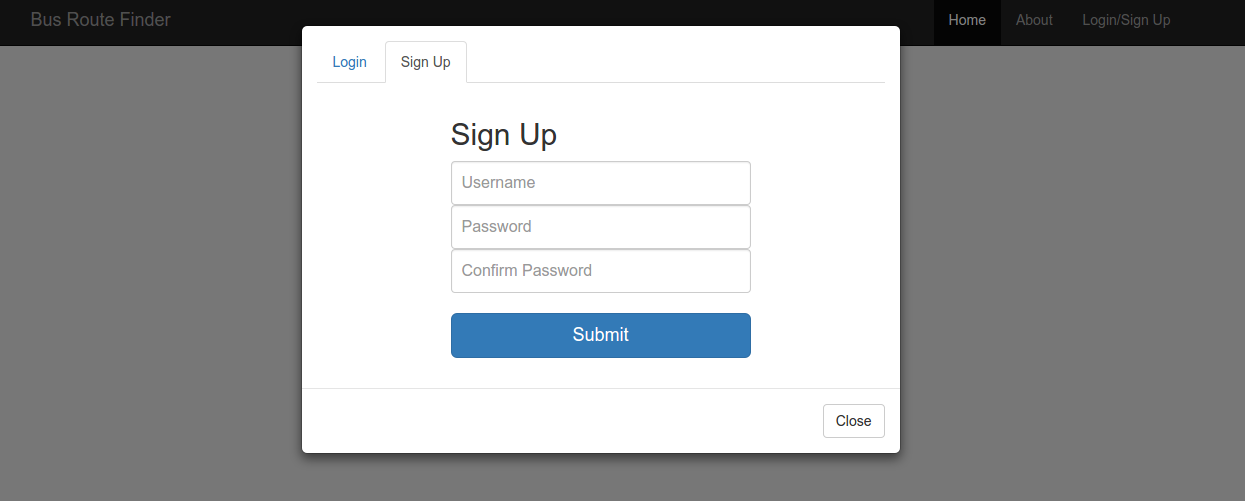
\includegraphics[scale = 0.38]{shots/signup.png}
\caption{Sign up page for a new user}
\label{overflow}
\end{figure}



\item \textbf{Admin Login} 

This will redirect to the admin interface which will allow the registry of a new bus. The details are mentioned in the bus registry page.

\end{itemize}

\item \textit{Selection of the bus/route from the set of paths outputted corresponding to the user input:}

This will give the set of the buses, the route, the travel time and the corresponding travel cost satisfying the input criteria sorted according to the travel time. In case of a transaction by the registered user, various discounts will also be reflected depending on the amount of bus transportation he has used in the past.

The discount formula is described as follows:
\begin{itemize}
\item If the total duration of bus journey exceeds 10 hrs, then only the user is eligible for discount.
\item If the above criteria is satisfied, then 
\begin{equation}
	 discount = 30\% * \frac{Total Journey Time}{Total Journey Time + 10 hrs}
\end{equation}

In this manner, the maximum discount that can be availed is 30\%.
\end{itemize}

\begin{figure}[ht!]
\center
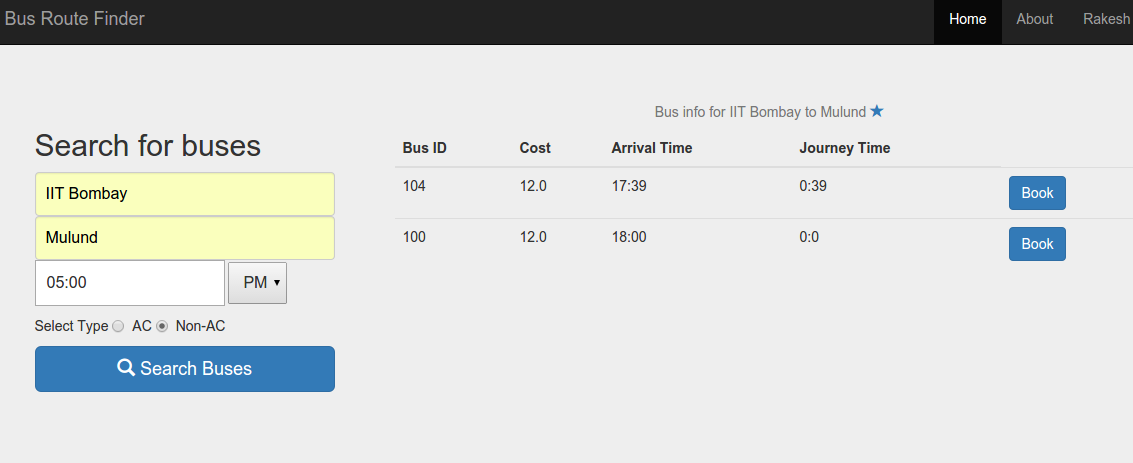
\includegraphics[scale = 0.4]{shots/fav.png}
\caption{The result of the transaction. Here the star button allows the registered user to mark it's favorite transactions}
\label{overflow}
\end{figure}



\item \textit{Bus Registry page:}

This page will enable a new bus service to be added. The admin will first add the source and starting time of the journey. Now the next hop of the journey should be adjacent to the source. This constraint will be implemented using a graph with nodes as bus-stops and edges as paths between them. The adjacency list of that source will be used for this and it would be enforced by an AJAX interface between front-end and back-end.

\begin{figure}[ht!]
\center{}
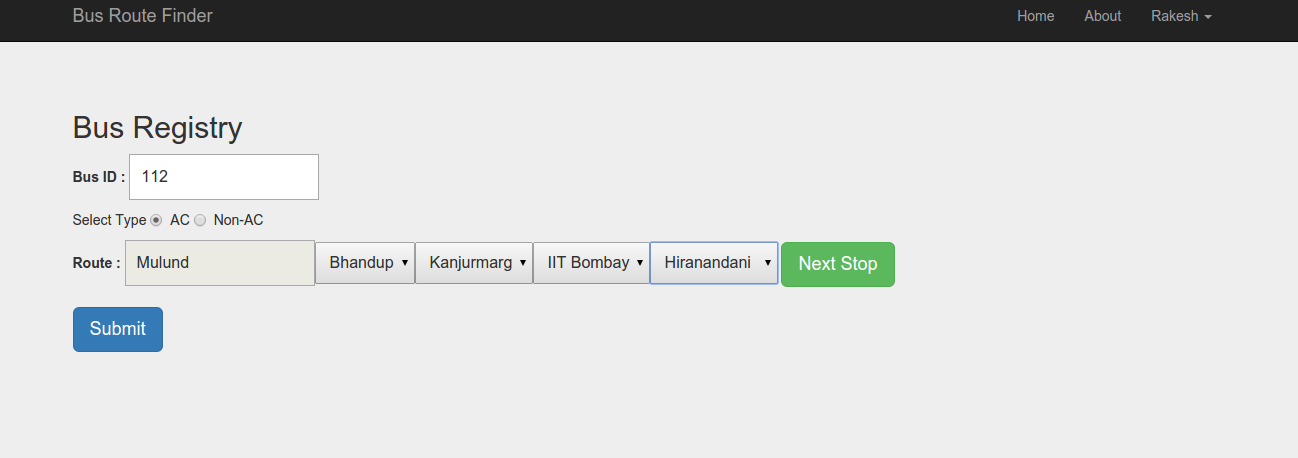
\includegraphics[scale = 0.38]{shots/regfinal.png}
\caption{The interactive bus registry page. Here the drop-down list of Hiranandani button contains the list of bus stops which can be further added in the route}
\label{overflow}
\end{figure}


\end{enumerate}

\pagebreak{}
\section{Data Model}
\paragraph{}
The data model of our database design is described by the following E-R model:

\begin{figure}[ht!]
\center
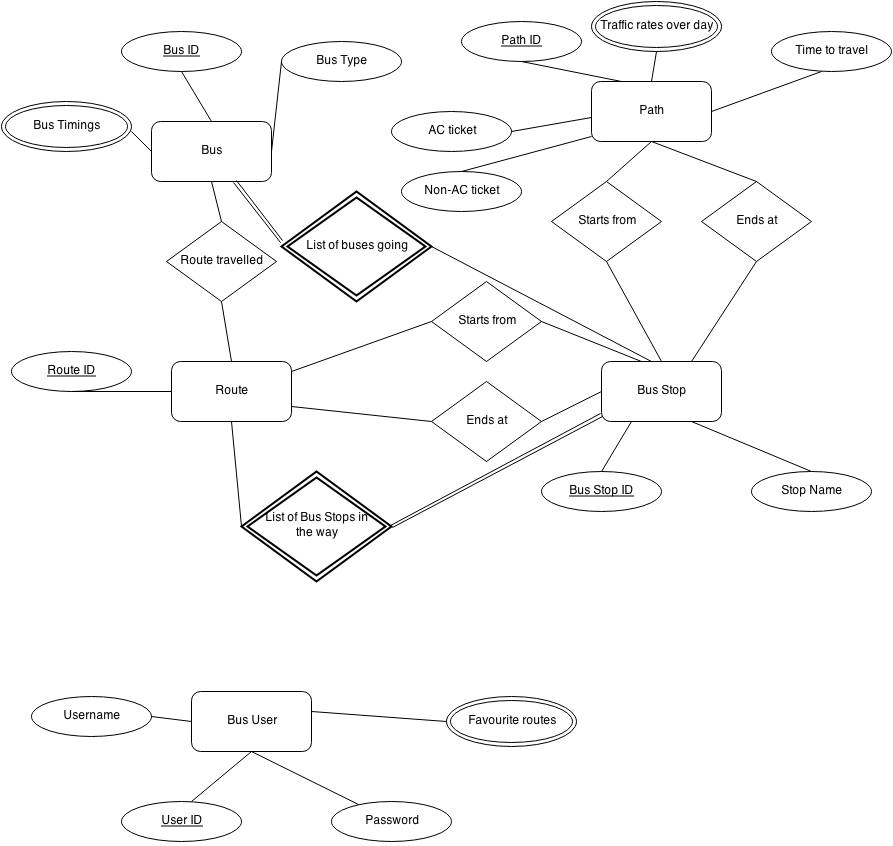
\includegraphics[width=150mm]{shots/er.jpg}
\caption{The Entity-Relationship Model/Data Model}
\label{overflow}
\end{figure}

\pagebreak{}

\section{Table Design}
\paragraph{}
The table design is depicted in the following diagram:

\begin{figure}[ht!]
\center
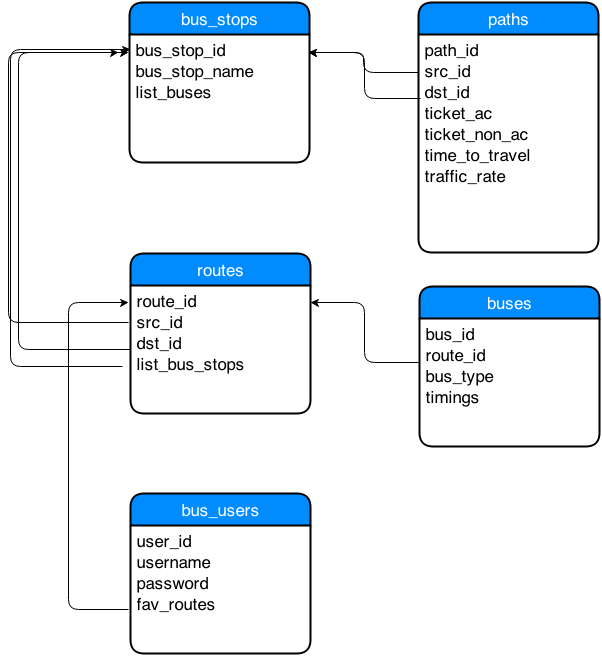
\includegraphics[width=150mm]{shots/table.png}
\caption{The Table Design}
\label{overflow}
\end{figure}
\pagebreak{}

\section{Conclusion}
\paragraph{}

In this project we learned about the various principles for constructing a web application. This included interaction with servlets and jsp. We learned how servlets interact with database to perform several queries on it and how they interact with client to serve these requests.

Apart from that we discovered how to optimize database operations in terms of space and time using normalization, indexing etc.


\pagebreak{}

\begin{thebibliography}{9}
\bibitem{bstrap}
http://getbootstrap.com/
\bibitem{jquery}
	http://jquery.com/
\end{thebibliography}


\end{document}
